
%(BEGIN_QUESTION)
% Copyright 2010, Tony R. Kuphaldt, released under the Creative Commons Attribution License (v 1.0)
% This means you may do almost anything with this work of mine, so long as you give me proper credit

Suppose we wish to have three separate pushbutton start/stop stations for operators to use in controlling a single three-phase electric motor.  The control circuit wiring schematic shows how this will work:

$$\includegraphics[width=15.5cm]{i02449x01.eps}$$

Sketch the necessary connecting wires to build this control circuit:

$$\includegraphics[width=15.5cm]{i02449x02.eps}$$

\vskip 20pt \vbox{\hrule \hbox{\strut \vrule{} {\bf Suggestions for Socratic discussion} \vrule} \hrule}

\begin{itemize}
\item{} An overload contact has been omitted from this motor control system for simplicity's sake.  Identify where one would be properly inserted into the schematic diagram, and also in the pictorial diagram.
\item{} After you have sketched wires to make a complete diagram, try to predict the effects of various faults in the circuit (e.g. switch contacts failing open or shorted ; wires breaking).
\end{itemize}

\underbar{file i02449}
%(END_QUESTION)





%(BEGIN_ANSWER)

$$\includegraphics[width=15.5cm]{i02449x03.eps}$$

%(END_ANSWER)





%(BEGIN_NOTES)


%INDEX% Electronics review: AC motor control circuit

%(END_NOTES)

